% From Ideas to Action: three agents, three problems
% Compile with XeLaTeX:  latexmk -xelatex ideas_to_action.tex
\documentclass[aspectratio=169,11pt,t]{beamer}

% ---------------------------------------------------------------- fonts
\usefonttheme{professionalfonts}
\usefonttheme{serif}
\usepackage{fontspec}
\usepackage{unicode-math}
\setmainfont{STIX Two Text}[BoldFont={STIXGeneral-Bold},BoldItalicFont={STIXGeneral-BoldItalic}]
\setmathfont{STIX Two Math}

\usepackage{booktabs,mathtools,tikz}
\usepackage{etoolbox}
\appto\normalsize{\setlength{\abovedisplayskip}{8pt}\setlength{\belowdisplayskip}{8pt}\setlength{\abovedisplayshortskip}{5pt}\setlength{\belowdisplayshortskip}{5pt}}
\usetikzlibrary{arrows.meta}

% --------------------------------------------------------------- colours
\definecolor{ink}{HTML}{222222}
\definecolor{muted}{HTML}{6E6E6E}
\definecolor{hair}{HTML}{BBBBBB}
\definecolor{nap}{HTML}{9A6A1F}   % Napoleon, vision
\definecolor{ber}{HTML}{2F5D8A}   % Berthier, AI
\definecolor{lan}{HTML}{3D7357}   % Lannes, physical progress

% ---------------------------------------------------------- beamer theme
\setbeamertemplate{navigation symbols}{}
\setbeamercolor{normal text}{fg=ink,bg=white}
\setbeamercolor{structure}{fg=ink}
\setbeamercolor{frametitle}{fg=ink}
\setbeamertemplate{itemize items}{\textendash}
\setbeamertemplate{enumerate item}{\insertenumlabel.}
\setlength{\leftmargini}{1.2em}
\setbeamersize{text margin left=1.4cm,text margin right=1.4cm}

\setbeamertemplate{frametitle}{%
  \vspace*{0.75cm}%
  {\fontsize{18}{21}\selectfont\insertframetitle}\par
  \vspace{0.45cm}}

\setbeamertemplate{footline}{%
  \hbox to \paperwidth{\hfill{\footnotesize\color{muted}\insertframenumber}\hspace{1.4cm}}%
  \vspace{0.45cm}}

% ------------------------------------------------------------ components
% agent names and key terms, colour-coded
\newcommand{\Nap}{\textcolor{nap}{Napoleon}}
\newcommand{\Ber}{\textcolor{ber}{Berthier}}
\newcommand{\Lan}{\textcolor{lan}{Lannes}}
\newcommand{\tN}[1]{\textcolor{nap}{\textbf{#1}}}
\newcommand{\tB}[1]{\textcolor{ber}{\textbf{#1}}}
\newcommand{\tL}[1]{\textcolor{lan}{\textbf{#1}}}
\newcommand{\tK}[1]{\textbf{#1}}
% headings and notes
\newcommand{\head}[2][ink]{{\itshape\color{#1}#2}\par\vspace{0.15cm}}
\newcommand{\aside}[1]{{\small\color{muted}#1\par}}
% key statement: larger type with a thin rule in the given colour
\newsavebox{\keysave}
\newenvironment{keypoint}[1][ink]{%
  \def\keycolor{#1}%
  \begin{lrbox}{\keysave}\begin{minipage}{\dimexpr\linewidth-0.7cm\relax}\raggedright\large\color{#1}}
  {\end{minipage}\end{lrbox}\par\noindent
  \begin{tikzpicture}[baseline=(k.north)]
    \node[inner sep=0pt,anchor=north west](k) at (0.55cm,0) {\usebox{\keysave}};
    \draw[\keycolor,line width=1.6pt] ([xshift=-0.4cm,yshift=2pt]k.north west) -- ([xshift=-0.4cm,yshift=-2pt]k.south west);
  \end{tikzpicture}\par}

\newcommand{\E}{\mathbb{E}}
\DeclareMathOperator{\tr}{tr}
\DeclareMathOperator{\Var}{Var}
\newcommand{\Ycal}{\mathcal{Y}}

\begin{document}

% ======================================================================= title
{\setbeamertemplate{footline}{}
\begin{frame}[plain,c]
  \hspace*{0.2cm}\begin{minipage}{0.8\textwidth}
  {\fontsize{28}{32}\selectfont From Ideas to Action}\par
  \vspace{0.35cm}
  {\large\itshape Three agents, three problems}\par
  \vspace{1.0cm}
  {\color{muted}October 2026}
  \end{minipage}
\end{frame}}

% ======================================================================= intro
\begin{frame}{Producing anything takes three kinds of work}
  \vspace{0.4cm}
  {\Large
  A \tN{strategist} decides \emph{what} to do.\par\vspace{0.35cm}
  A \tB{solver} works out \emph{how}.\par\vspace{0.35cm}
  An \tL{executor} \emph{does} it.\par}
  \vspace{0.8cm}
  \begin{keypoint}
    Which of the three can AI improve, and does that make the economy grow?
  \end{keypoint}
\end{frame}

\begin{frame}{Plans, actions, and value}
  A \tK{plan} $\xi$ says what to do. A detailed \tK{action} $a\in\mathcal{A}(\xi)$ carries it out and yields \tK{payoff} $W(a;\xi)$.
  \vspace{0.3cm}
  \[a^*(\xi)\in\arg\max_{a\in\mathcal{A}(\xi)}W(a;\xi),\qquad v(\xi)=W\big(a^*(\xi);\xi\big)\]
  \vspace{0.2cm}
  \begin{keypoint}
    $a^*(\xi)$ is the \tK{ideal solution}; $v(\xi)$ is the \tK{value} of the plan.
  \end{keypoint}
  \vspace{0.3cm}
  \aside{Throughout, every problem is smooth: $\mathcal{A}(\xi)\subset\mathbb{R}^d$ is compact and $W(\cdot\,;\xi)$ is infinitely differentiable ($C^\infty$) in $a$.}
\end{frame}

\begin{frame}{Three agents, three problems}
  \vspace{0.2cm}
  \centering
  \renewcommand{\arraystretch}{1.5}
  \begin{tabular}{@{}l l l l@{}}
    \toprule
    & Problem & Input & Output \\
    \midrule
    \textcolor{nap}{Strategist} & What should we do? & candidate plans & plan $\xi$ \\
    \textcolor{ber}{Solver} & Exactly how is $\xi$ done? & plan $\xi$ & solution $\hat a$ \\
    \textcolor{lan}{Executor} & Carry out $\hat a$ physically & solution $\hat a$ & action $\tilde a$ \\
    \bottomrule
  \end{tabular}\par
  \raggedright
  \vspace{0.7cm}
  \begin{keypoint}
    Output is $Y=W(\tilde a;\xi)$: the payoff of what actually gets done.
  \end{keypoint}
\end{frame}

% ======================================================================= reveal
\begin{frame}{Meet the three agents}
  \vspace{0.2cm}
  \begin{itemize}\setlength{\itemsep}{14pt}
    \item[] {\Large\textcolor{nap}{Napoleon}}\quad the strategist\par
      {\color{muted}decided what each campaign should achieve.}
    \item[] {\Large\textcolor{ber}{Berthier}}\quad the solver\par
      {\color{muted}his chief of staff: turned Napoleon's intentions into detailed orders, routes, and timetables.}
    \item[] {\Large\textcolor{lan}{Lannes}}\quad the executor\par
      {\color{muted}the marshal who carried those orders out on the battlefield.}
  \end{itemize}
  \vspace{0.3cm}
  \aside{From here on we call the three agents by their names.}
\end{frame}

% ======================================================================= strategist
\begin{frame}{Where candidate plans come from}
  Candidate plans are drawn independently, $\xi\sim F$. Each comes with its \emph{whole} payoff function $W(\cdot\,;\xi)$.
  \vspace{0.2cm}

  A plan's \tN{expected value} is computed from that function and from how it will be solved and carried out:
  \[U=u(\xi)=\E\big[W(\tilde a;\xi)\mid\xi\big].\]
  \begin{keypoint}
    $G$, the distribution of $U$, is \emph{induced}: by the pool of plans $F$, and by how well Berthier and Lannes handle each plan.
  \end{keypoint}
  \vspace{0.2cm}
  \aside{In general $G$ can be any distribution. It is normal only under the conditions of the Gaussian example below.}
\end{frame}

\begin{frame}{The \textcolor{nap}{strategist} investigates before choosing}
  \head[nap]{Definition 1 (Strategist, or Napoleon)}
  A strategist, or a \Nap, is a pair $N=(\tau_s,\mathcal{S})$:
  \begin{itemize}\setlength{\itemsep}{6pt}
    \item \tN{signal technology} $\mathcal{S}=\{P(\cdot\mid u)\}_u$: signals $s_1,s_2,\dots\in\Sigma$ about a plan's expected value $U\sim G$, i.i.d.\ given $U$;
    \item \tN{signal time} $\tau_s$: how long each signal takes.
  \end{itemize}
  \vspace{0.4cm}
  \begin{keypoint}[nap]
    Plans are plentiful. Time to learn which are good is scarce.
  \end{keypoint}
  \vspace{0.2cm}
  \aside{Napoleon judges what a plan will actually deliver, after the losses in solving and doing it, not its ideal value.}
\end{frame}

\begin{frame}{A policy says when to stop investigating}
  A \tN{policy} is a decision after every history of signals:
  \[\pi=(\pi_n)_{n\ge1},\qquad\pi_n:\Sigma^n\to\{\text{accept},\ \text{reject},\ \text{wait}\}.\]
  It stops after $N_\pi=\min\{n:\pi_n(s_1,\dots,s_n)\ne\text{wait}\}$ signals.
  \vspace{0.3cm}

  $\Pi$ is the set of policies with $\E[N_\pi]<\infty$.
\end{frame}

\begin{frame}{\Nap's problem}
  \head[nap]{Problem N (investigation)}
  \[\max_{\pi\in\Pi}\ Q(\pi)\,\E_\pi[U\mid\text{accept}]\qquad\text{s.t.}\qquad Q(\pi)\le K\]
  \aside{By iterated expectations, $\E_\pi[Y\mid\text{accept}]=\E_\pi[U\mid\text{accept}]$.}
  \vspace{0.3cm}
  \begin{keypoint}[nap]
    Waiting buys information about one plan, but leaves less time for others.
  \end{keypoint}
\end{frame}

\begin{frame}{Flows and capacity}
  \tN{Accepted flow}: plans accepted per unit of time by $n_A$ Napoleons,
  \[Q(\pi)=\frac{n_A\,P_\pi(\text{accept})}{\tau_s\,\E_\pi[N_\pi]}.\]
  \tK{Downstream capacity}: plans per unit of time that $n_B$ Berthiers and $n_L$ Lannes can handle,
  \[K=\min\Big\{\frac{n_B}{\tau_B},\ \frac{n_L}{\tau_L}\Big\}.\]
  \aside{$Q(\pi)$ is a rate: $n_A/\tau_s$ signals per unit of time, divided by $\E_\pi[N_\pi]$ signals per plan, times the share accepted. Derivation in the appendix.}
\end{frame}

% ======================================================================= solver
\begin{frame}{The \textcolor{ber}{solver} works out the details}
  \head[ber]{Definition 2 (Solver, or Berthier)}
  A solver, or a \Ber, is a pair $B=(\tau_B,k)$. Berthier replaces the true payoff with its best approximation from a \tB{sieve} $\mathcal{W}_k$, a family of functions of complexity $k$:
  \[\hat W(\cdot\,;\xi)\in\arg\min_{f\in\mathcal{W}_k}\ \sup_{a\in\mathcal{A}(\xi)}\big|f(a)-W(a;\xi)\big|.\]
  \begin{itemize}\setlength{\itemsep}{6pt}
    \item \tB{sieve size} $k$: how rich a model Berthier can handle;
    \item \tB{solving time} $\tau_B$ per plan, so plans are solved at rate $\mu_B=n_B/\tau_B$.
  \end{itemize}
\end{frame}

\begin{frame}{A richer sieve is a better approximation}
  The \tB{approximation error} is the distance from $W$ to the sieve:
  \[\varepsilon_B(k)\equiv\min_{f\in\mathcal{W}_k}\ \sup_{a\in\mathcal{A}(\xi)}\big|f(a)-W(a;\xi)\big|.\]
  For standard sieves (polynomials, splines) and $W\in C^s$, approximation theory gives
  \[\varepsilon_B(k)\ \le\ C_s\,k^{-s/d}\qquad\text{for every }s,\text{ since }W\in C^\infty.\]
  \begin{keypoint}[ber]
    The approximation is global: it does not depend on knowing where the optimum is.
  \end{keypoint}
  \vspace{0.05cm}
  \aside{$C_s$ depends on bounds on the first $s$ derivatives of $W$. Neural networks are sieves too. The rate worsens with the number of decision variables $d$.}
\end{frame}

\begin{frame}{\Ber's problem}
  \head[ber]{Problem B (approximate, then solve)}
  Solve the approximate problem exactly:
  \[\hat{\mathcal{P}}(\xi):\quad\hat a\in\arg\max_{a\in\mathcal{A}(\xi)}\hat W(a;\xi).\]
  \tB{Solution loss}: what the approximation costs in the true problem,
  \[\kappa_B(\xi)=\big|v(\xi)-W(\hat a;\xi)\big|=v(\xi)-W(\hat a;\xi).\]
  \aside{The two agree because $v(\xi)$ is the maximum, so $W(\hat a;\xi)\le v(\xi)$.}
  \begin{keypoint}[ber]
    Berthier errs in his model of the problem, never in the goal.
  \end{keypoint}
\end{frame}

\begin{frame}{A good approximation gives a good solution}
  \head{Lemma 1 (approximation bound)}
  {\itshape If Berthier's approximation is within $\varepsilon_B(k)$ of the true payoff, then}
  \[\kappa_B(\xi)\ \le\ 2\,\varepsilon_B(k)\ \le\ 2\,C_s\,k^{-s/d}.\]
  \begin{keypoint}[ber]
    Solution loss is at most twice the approximation error, whatever the problem.
  \end{keypoint}
\end{frame}

% ======================================================================= executor
\begin{frame}{The \textcolor{lan}{executor} carries out the solution}
  \head[lan]{Definition 3 (Executor, or Lannes)}
  An executor, or a \Lan, is a pair $L=(\tau_L,\mathcal{R})$:
  \begin{itemize}\setlength{\itemsep}{6pt}
    \item \tL{budget set} $\mathcal{R}\subseteq\mathcal{A}(\xi)$: the actions that can physically be carried out;
    \item \tL{execution time} $\tau_L$ per plan, so plans are carried out at rate $\mu_L=n_L/\tau_L$.
  \end{itemize}
  \vspace{0.3cm}
  \begin{keypoint}[lan]
    Berthier's solution $\hat a$ need not lie in $\mathcal{R}$.
  \end{keypoint}
\end{frame}

\begin{frame}{\Lan's problem}
  \head[lan]{Problem L (execution)}
  Carry out the feasible action closest to Berthier's solution:
  \[\tilde a=\arg\min_{r\in\mathcal{R}}\ \lVert r-\hat a\rVert.\]
  \tL{Execution loss}: zero whenever $\hat a\in\mathcal{R}$,
  \[\kappa_L(\xi)=\E\big[W(\hat a;\xi)-W(\tilde a;\xi)\mid\xi\big].\]
  \tL{Best feasible value}: $\bar U(\xi)=\max_{r\in\mathcal{R}}W(r;\xi)\le v(\xi)$.
\end{frame}

% ======================================================================= together
\begin{frame}{Output depends on all three}
  \vspace{0.3cm}
  \centering
  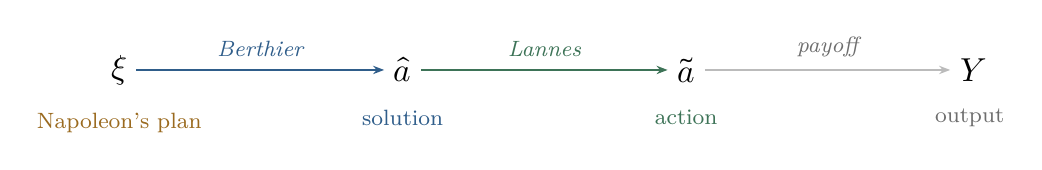
\begin{tikzpicture}[
      arr/.style={-{Stealth[length=4pt]},line width=0.7pt},
      lab/.style={font=\footnotesize\itshape,above=1pt},
      capt/.style={font=\footnotesize,below=3pt}]
    \node(i) at (0,0)    {\large$\xi$};
    \node(a) at (3.6,0)  {\large$\hat a$};
    \node(x) at (7.2,0)  {\large$\tilde a$};
    \node(y) at (10.8,0) {\large$Y$};
    \draw[arr,ber] (i) -- node[lab,text=ber]{Berthier} (a);
    \draw[arr,lan] (a) -- node[lab,text=lan]{Lannes} (x);
    \draw[arr,hair] (x) -- node[lab,text=muted]{payoff} (y);
    \node[capt,text=nap] at (i.south) {Napoleon's plan};
    \node[capt,text=ber] at (a.south) {solution};
    \node[capt,text=lan] at (x.south) {action};
    \node[capt,text=muted] at (y.south) {output};
  \end{tikzpicture}\par
  \vspace{0.2cm}
  \[U\;=\;\E[Y\mid\xi]\;=\;\textcolor{nap}{v(\xi)}\;-\;\textcolor{ber}{\kappa_B(\xi)}\;-\;\textcolor{lan}{\kappa_L(\xi)}\]
  \raggedright
  \vspace{0.2cm}
  \begin{keypoint}
    Expected value: \textcolor{nap}{ideal value}, minus \textcolor{ber}{what is lost solving it}, minus \textcolor{lan}{what is lost doing it}.
  \end{keypoint}
\end{frame}

\begin{frame}{A local view of the losses}
  Near the ideal solution, with $d=a-a^*(\xi)$:
  \[W(a;\xi)\approx v(\xi)-\tfrac12\,d^{\top}H\,d,\qquad H=-\nabla_a^2W\big(a^*(\xi);\xi\big).\]
  If Berthier's approximation puts the optimum at $\hat a=a^*(\xi)+\delta_B$, his loss is $\textcolor{ber}{\kappa_B=\tfrac12\delta_B^{\top}H\delta_B}$. Lannes's loss is the cost of moving $\hat a$ into $\mathcal{R}$.
  \vspace{0.2cm}
  \begin{keypoint}
    \textcolor{ber}{Berthier's loss comes from approximation}; \textcolor{lan}{Lannes's loss comes from infeasibility}.
  \end{keypoint}
\end{frame}

\begin{frame}{Example: Gaussian plans}
  Suppose plans differ only in their \emph{level}: a common shape $w$, with $\max_aw(a)=0$, and a normal ideal value,
  \[W(a;\xi)=v(\xi)+w(a),\qquad v(\xi)\sim N(m,\sigma^2).\]
  Shifting $W$ by a constant moves neither Berthier's sieve solution $\hat a$ nor Lannes's action $\tilde a$, so both losses are the same for every plan:
  \[U=v(\xi)-\kappa_B-\kappa_L\ \sim\ N\big(m-\kappa,\ \sigma^2\big).\]
  \aside{This needs the sieve to contain constant functions, as polynomials and splines do.}
\end{frame}

\begin{frame}{Example: Gaussian signals}
  Under the Gaussian-plans conditions, $U\sim N(m-\kappa,\sigma^2)$. Signals are normal around it:
  \[s_k=U+\eta_k,\qquad\eta_k\sim N(0,\sigma_\eta^2).\]
  After $n$ signals, Napoleon's estimate of $U$ is the posterior mean
  \[\mu_n\sim N\big(m-\kappa,\ \rho_n\sigma^2\big),\qquad\rho_n=\frac{n}{n+r},\qquad r=\frac{\sigma_\eta^2}{\sigma^2}.\]
  \aside{$\rho_n$ is the \emph{accuracy} of the estimate. Below, $m_U=m-\kappa$ and $\sigma_U=\sigma$.}
\end{frame}

\begin{frame}{$Q$ in the Gaussian case}
  Take $n$ signals, then accept if the posterior mean clears a cutoff, $\mu_n\ge z$ (chosen on the next slide). The estimate is
  \[\mu_n=m_U+\rho_n(\bar s_n-m_U),\qquad \bar s_n=\tfrac1n\textstyle\sum_{k\le n}s_k\sim N\big(m_U,\ \sigma_U^2+\sigma_\eta^2/n\big),\]
  so $\Var(\mu_n)=\rho_n^2(\sigma_U^2+\sigma_\eta^2/n)=\rho_n\sigma_U^2$. With $N_\pi=n$,
  \[P_\pi(\text{accept})=1-\Phi\!\Big(\frac{z-m_U}{\sigma_U\sqrt{\rho_n}}\Big),\qquad Q(\pi)=\frac{n_A}{n\,\tau_s}\Big[1-\Phi\Big(\frac{z-m_U}{\sigma_U\sqrt{\rho_n}}\Big)\Big].\]
  \aside{Year 0 of the illustration: $n=3$, $z\approx0.21$, $P_\pi(\text{accept})=0.15$, and $Q=0.15/(3\times0.05)=1$ plan a year $=K$.}
\end{frame}

\begin{frame}{\Nap's trade-off: how selective he can be}
  With $n$ signals per plan, each plan takes $n\tau_s$. So $n_A$ Napoleons examine
  \[R_n=\frac{n_A}{n\,\tau_s}\quad\text{plans per unit of time.}\]
  Capacity lets $K$ of them through, so Napoleon accepts the top share $q_n=K/R_n=Kn\tau_s/n_A$. He does so with a \tN{cutoff} on his estimate, never accepting a plan worth less than nothing:
  \[\text{accept}\iff\mu_n\ge z_n,\qquad z_n=\max\Big\{0,\ m_U+\sigma_U\sqrt{\rho_n}\,\Phi^{-1}(1-q_n)\Big\}.\]
  \begin{keypoint}[nap]
    More signals per plan: fewer plans examined, so Napoleon must be less selective.
  \end{keypoint}
\end{frame}

\begin{frame}{\Nap's trade-off: how good his picks are}
  Napoleon accepts the plans with the highest estimates $\mu_n$. Since $\E[U\mid\mu_n]=\mu_n$,
  \[\E[U\mid\text{accept}]=\E\big[\mu_n\ \big|\ \mu_n\text{ in its top share }q_n\big].\]
  Under the Gaussian-plans conditions, $\mu_n=m_U+\sigma_U\sqrt{\rho_n}\,X$ with $X\sim N(0,1)$. The top share $q$ of $X$ has mean $S(q)=\phi\big(\Phi^{-1}(1-q)\big)/q$, so
  \[\E[U\mid\text{accept}]=m_U+\sigma_U\sqrt{\rho_n}\;S(q_n).\]
  \aside{$S(q)$ is the inverse Mills ratio: $S(0.05)=2.06$, $S(0.15)=1.55$, $S(0.5)=0.80$, $S(1)=0$.}
\end{frame}

\begin{frame}{\Nap's trade-off: output}
  Output is the accepted flow times the value of each accepted plan:
  \[\Ycal(n)=K\Big(m_U+\sigma_U\,\sqrt{\rho_n}\;S(q_n)\Big).\]
  \begin{itemize}\setlength{\itemsep}{2pt}
    \item $K$: plans carried out per unit of time;
    \item $m_U$: the value of an average plan;
    \item $\sigma_U$: how much plans differ, i.e.\ what there is to gain from choosing well;
    \item \tN{$\sqrt{\rho_n}$}: how much of that difference Napoleon can see after $n$ signals;
    \item \tN{$S(q_n)$}: how far above average, in standard deviations, the plans he picks are.
  \end{itemize}
  \aside{Assumes capacity binds and the cutoff is positive; otherwise Napoleon accepts fewer than $K$ plans.}
\end{frame}

\begin{frame}{Choosing $n$: year 0 of the illustration}
  \centering
  \renewcommand{\arraystretch}{1.1}
  \begin{tabular}{@{}c r r r r r@{}}
    \toprule
    $n$ & $R_n$ & $q_n$ & $\sqrt{\rho_n}$ & $S(q_n)$ & $\Ycal(n)$ \\
    {\footnotesize\color{muted}signals} & {\footnotesize\color{muted}examined} & {\footnotesize\color{muted}share accepted} & {\footnotesize\color{muted}accuracy} & {\footnotesize\color{muted}selectivity} & {\footnotesize\color{muted}output} \\
    \midrule
    1 & 20.0 & 0.05 & 0.45 & 2.06 & 1.19 \\
    2 & 10.0 & 0.10 & 0.58 & 1.76 & 1.55 \\
    \textbf{3} & \textbf{6.7} & \textbf{0.15} & \textbf{0.65} & \textbf{1.55} & \textbf{1.57} \\
    4 & 5.0 & 0.20 & 0.71 & 1.40 & 1.46$^*$ \\
    \bottomrule
  \end{tabular}\par
  \raggedright
  \vspace{0.2cm}
  \begin{keypoint}[nap]
    Napoleon takes 3 signals: with fewer he cannot tell plans apart; with more he sees too few plans.
  \end{keypoint}
  \vspace{0.1cm}
  \aside{$m_U=-2.5$, $\sigma_U=4$, $r=4$, $\tau_s=0.05$, $n_A=K=1$. $^*$Cutoff hits zero: fewer than $K$ accepted.}
\end{frame}

% ======================================================================= AI, vision, RSI
\begin{frame}{AI is a better \Ber}
  \head[ber]{Definition 4 (AI)}
  \tB{AI} is an improvement to Berthier:
  \[\tau_B'\le\tau_B\qquad\text{or}\qquad k'\ge k.\]
  \vspace{0.2cm}
  \begin{keypoint}[ber]
    Faster solving ($\mu_B\uparrow$) or richer approximations ($\varepsilon_B\downarrow$, a tighter bound on $\kappa_B$).
  \end{keypoint}
\end{frame}

\begin{frame}{Vision is a better \Nap}
  \head[nap]{Definition 5 (Vision)}
  \tN{Vision} is an improvement to Napoleon:
  \[\tau_s'\le\tau_s\qquad\text{or}\qquad\mathcal{S}'\ \text{Blackwell more informative than}\ \mathcal{S}.\]
  \vspace{0.2cm}
  \begin{keypoint}[nap]
    Faster screening of plans, or sharper judgment about them.
  \end{keypoint}
\end{frame}

\begin{frame}{RSI is both}
  \head{Definition 6 (RSI)}
  \tK{RSI} is AI and vision together: a better \Ber{} and a better \Nap.
  \vspace{0.5cm}
  \begin{keypoint}[lan]
    In all three cases, Lannes is unchanged.
  \end{keypoint}
\end{frame}

% ======================================================================= results
\begin{frame}{Assumptions behind the results}
  \begin{enumerate}\setlength{\itemsep}{6pt}
    \item \Lan{} is fixed: $\tau_L$ and $\mathcal{R}$ do not change.
    \item $\E|v(\xi)|<\infty$, and output starts positive.
    \item For Results 2--3: best feasible values $\max_{r\in\mathcal{R}}W(r;\xi)$ have thin tails ($\sigma$-sub-Gaussian around their mean); and screening outpaces capacity, $n_A/\tau_s\ge\sqrt e\,n_L/\tau_L$.
  \end{enumerate}
  \vspace{0.3cm}
  \begin{keypoint}[lan]
    Whatever Berthier does, the action lies in $\mathcal{R}$, so $U\le\max_{r\in\mathcal{R}}W(r;\xi)$.
  \end{keypoint}
  \vspace{0.2cm}
  \aside{Output growth rate: $g_{\Ycal}=\limsup_t\frac1t\ln\Ycal_t$. Proofs are in the appendix.}
\end{frame}

\begin{frame}{Result 1: AI alone cannot sustain growth}
  \head{Proposition 1}
  {\itshape Fix Napoleon and Lannes. Along any path of AI, for all $t$,}
  \[\Ycal_t\ \le\ \frac{n_A}{\tau_s}\;\E_{\xi\sim F}\Big[\max\Big\{0,\ \max_{r\in\mathcal{R}}W(r;\xi)\Big\}\Big]\ <\ \infty.\]
  \begin{keypoint}[ber]
    AI raises output at most to a fixed ceiling, then stops.
  \end{keypoint}
  \vspace{0.2cm}
  \aside{$n_A/\tau_s$: the fastest rate of examining plans. $\max_{r\in\mathcal{R}}W(r;\xi)$: the plan's best feasible value. Neither depends on Berthier.}
\end{frame}

\begin{frame}{No information beats perfect sorting}
  \head{Lemma 2 (selection bound)}
  {\itshape Let $Z-\E[Z]$ be $\sigma$-sub-Gaussian, and let $A$ be any event with $P(A)=q$, such as ``Napoleon accepts the plan''. Then}
  \[\E[Z\mid A]\ \le\ \E[Z]+\sigma\sqrt{2\ln(1/q)}.\]
  \begin{keypoint}[nap]
    Being more selective helps, but only like $\sqrt{\ln(1/q)}$.
  \end{keypoint}
  \vspace{0.2cm}
  \aside{Applied with $Z=\max_{r\in\mathcal{R}}W(r;\xi)$, it bounds the plans Napoleon accepts under any signals and any policy.}
\end{frame}

\begin{frame}{Result 2: sharper judgment has a ceiling}
  \head{Proposition 2}
  {\itshape Fix the signal time $\tau_s$. For any Berthier and any signal technology, even perfect information,}
  \[\Ycal\ \le\ K\bigg(\max\Big\{0,\ \E_{\xi\sim F}\Big[\max_{r\in\mathcal{R}}W(r;\xi)\Big]\Big\}+\sigma\sqrt{2\ln\frac{n_A}{K\tau_s}}\bigg).\]
  \begin{keypoint}[nap]
    Better judgment can at best reach full information.
  \end{keypoint}
\end{frame}

\begin{frame}{Result 3: thin tails stop all growth}
  \head{Proposition 3}
  {\itshape If signals speed up at most exponentially, $\tau_{s,t}\ge\tau_{s,0}e^{-gt}$, then for any AI and any vision}
  \[\Ycal_t\ \le\ \frac{n_L}{\tau_L}\bigg(\max\Big\{0,\ \E_{\xi\sim F}\Big[\max_{r\in\mathcal{R}}W(r;\xi)\Big]\Big\}+\sigma\sqrt{2\ln\frac{n_A\tau_L}{n_L\tau_{s,0}}+2gt}\bigg).\]
  \begin{keypoint}
    Output grows at most like $\sqrt t$: \textcolor{ber}{AI}, \textcolor{nap}{vision}, and RSI all level off.
  \end{keypoint}
\end{frame}

\begin{frame}{Heavy tails change this}
  Suppose expected values have a Pareto tail, $P(U>x)=(x/x_m)^{-\alpha}$ with $\alpha>1$. Then the best plans improve as a power of the pool screened:
  \[M(q)=\tfrac{\alpha}{\alpha-1}\,x_m\,q^{-1/\alpha},\qquad g_{\Ycal}\ \le\ g/\alpha,\]
  with equality under perfectly informative signals.
  \vspace{0.2cm}
  \begin{keypoint}[nap]
    Lasting growth from vision needs faster screening \emph{and} rare, enormously valuable plans.
  \end{keypoint}
\end{frame}

% ======================================================================= illustration
\begin{frame}{An illustration}
  \vspace{0.2cm}
  \centering
  \renewcommand{\arraystretch}{1.45}
  \begin{tabular}{@{}l l l@{}}
    \toprule
    & Year 0 & Each year after \\
    \midrule
    \Nap & $m=0$, $\sigma=4$, $r=4$, $\tau_s=0.05$ & \textcolor{nap}{vision}: $\tau_s$, $r$ divided by 1.1 \\
    \Ber & $\mu_B=1$, $\kappa_B=1.5$ & \textcolor{ber}{AI}: $\mu_B\times1.25$, $\kappa_B\div1.25$ (rising $k$) \\
    \Lan & $\mu_L=2$, $\kappa_L=1$ & unchanged \\
    \bottomrule
  \end{tabular}\par
  \raggedright
  \vspace{0.5cm}
  \aside{One Napoleon ($n_A=1$). Gaussian plans, so both losses are constants and $U\sim N(-\kappa,4^2)$. Napoleon re-chooses the number of signals each year. Illustrative parameters, not a forecast.}
\end{frame}

\begin{frame}{With thin tails, every path levels off}
  \vspace{0.1cm}
  \centering
  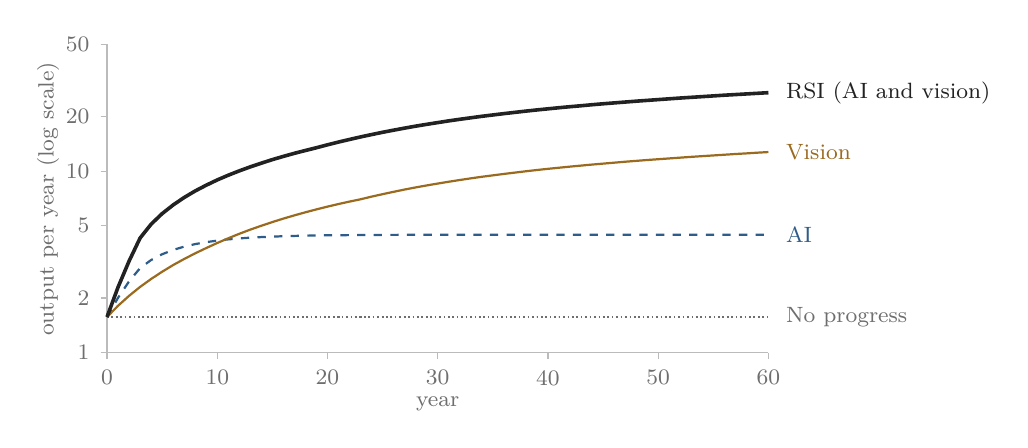
\begin{tikzpicture}
    \draw[hair,line width=0.4pt] (0,0) -- (0,3.912);
    \draw[hair,line width=0.4pt] (0,0) -- (8.400,0);
    \draw[hair,line width=0.4pt] (-0.08,0.000) -- (0,0.000); \node[anchor=east,font=\footnotesize,text=muted] at (-0.1,0.000) {1};
    \draw[hair,line width=0.4pt] (-0.08,0.693) -- (0,0.693); \node[anchor=east,font=\footnotesize,text=muted] at (-0.1,0.693) {2};
    \draw[hair,line width=0.4pt] (-0.08,1.609) -- (0,1.609); \node[anchor=east,font=\footnotesize,text=muted] at (-0.1,1.609) {5};
    \draw[hair,line width=0.4pt] (-0.08,2.303) -- (0,2.303); \node[anchor=east,font=\footnotesize,text=muted] at (-0.1,2.303) {10};
    \draw[hair,line width=0.4pt] (-0.08,2.996) -- (0,2.996); \node[anchor=east,font=\footnotesize,text=muted] at (-0.1,2.996) {20};
    \draw[hair,line width=0.4pt] (-0.08,3.912) -- (0,3.912); \node[anchor=east,font=\footnotesize,text=muted] at (-0.1,3.912) {50};
    \draw[hair,line width=0.4pt] (0.000,0) -- (0.000,-0.08); \node[anchor=north,font=\footnotesize,text=muted] at (0.000,-0.1) {0};
    \draw[hair,line width=0.4pt] (1.400,0) -- (1.400,-0.08); \node[anchor=north,font=\footnotesize,text=muted] at (1.400,-0.1) {10};
    \draw[hair,line width=0.4pt] (2.800,0) -- (2.800,-0.08); \node[anchor=north,font=\footnotesize,text=muted] at (2.800,-0.1) {20};
    \draw[hair,line width=0.4pt] (4.200,0) -- (4.200,-0.08); \node[anchor=north,font=\footnotesize,text=muted] at (4.200,-0.1) {30};
    \draw[hair,line width=0.4pt] (5.600,0) -- (5.600,-0.08); \node[anchor=north,font=\footnotesize,text=muted] at (5.600,-0.1) {40};
    \draw[hair,line width=0.4pt] (7.000,0) -- (7.000,-0.08); \node[anchor=north,font=\footnotesize,text=muted] at (7.000,-0.1) {50};
    \draw[hair,line width=0.4pt] (8.400,0) -- (8.400,-0.08); \node[anchor=north,font=\footnotesize,text=muted] at (8.400,-0.1) {60};
    \draw[densely dotted,muted,line width=0.6pt] plot coordinates {(0.000,0.451) (0.140,0.451) (0.280,0.451) (0.420,0.451) (0.560,0.451) (0.700,0.451) (0.840,0.451) (0.980,0.451) (1.120,0.451) (1.260,0.451) (1.400,0.451) (1.540,0.451) (1.680,0.451) (1.820,0.451) (1.960,0.451) (2.100,0.451) (2.240,0.451) (2.380,0.451) (2.520,0.451) (2.660,0.451) (2.800,0.451) (2.940,0.451) (3.080,0.451) (3.220,0.451) (3.360,0.451) (3.500,0.451) (3.640,0.451) (3.780,0.451) (3.920,0.451) (4.060,0.451) (4.200,0.451) (4.340,0.451) (4.480,0.451) (4.620,0.451) (4.760,0.451) (4.900,0.451) (5.040,0.451) (5.180,0.451) (5.320,0.451) (5.460,0.451) (5.600,0.451) (5.740,0.451) (5.880,0.451) (6.020,0.451) (6.160,0.451) (6.300,0.451) (6.440,0.451) (6.580,0.451) (6.720,0.451) (6.860,0.451) (7.000,0.451) (7.140,0.451) (7.280,0.451) (7.420,0.451) (7.560,0.451) (7.700,0.451) (7.840,0.451) (7.980,0.451) (8.120,0.451) (8.260,0.451) (8.400,0.451)};
    \node[anchor=west,font=\footnotesize,text=muted] at (8.500,0.451) {No progress};
    \draw[dashed,ber,line width=0.8pt] plot coordinates {(0.000,0.451) (0.140,0.695) (0.280,0.904) (0.420,1.072) (0.560,1.175) (0.700,1.248) (0.840,1.303) (0.980,1.345) (1.120,1.377) (1.260,1.402) (1.400,1.421) (1.540,1.437) (1.680,1.449) (1.820,1.459) (1.960,1.466) (2.100,1.472) (2.240,1.477) (2.380,1.481) (2.520,1.484) (2.660,1.487) (2.800,1.489) (2.940,1.490) (3.080,1.491) (3.220,1.492) (3.360,1.493) (3.500,1.494) (3.640,1.494) (3.780,1.495) (3.920,1.495) (4.060,1.495) (4.200,1.496) (4.340,1.496) (4.480,1.496) (4.620,1.496) (4.760,1.496) (4.900,1.496) (5.040,1.496) (5.180,1.496) (5.320,1.496) (5.460,1.496) (5.600,1.496) (5.740,1.496) (5.880,1.496) (6.020,1.496) (6.160,1.496) (6.300,1.496) (6.440,1.496) (6.580,1.496) (6.720,1.496) (6.860,1.496) (7.000,1.496) (7.140,1.496) (7.280,1.496) (7.420,1.496) (7.560,1.496) (7.700,1.496) (7.840,1.496) (7.980,1.496) (8.120,1.496) (8.260,1.496) (8.400,1.496)};
    \node[anchor=west,font=\footnotesize,text=ber] at (8.500,1.496) {AI};
    \draw[nap,line width=0.8pt] plot coordinates {(0.000,0.451) (0.140,0.594) (0.280,0.720) (0.420,0.833) (0.560,0.934) (0.700,1.026) (0.840,1.111) (0.980,1.188) (1.120,1.260) (1.260,1.327) (1.400,1.391) (1.540,1.451) (1.680,1.508) (1.820,1.561) (1.960,1.610) (2.100,1.657) (2.240,1.701) (2.380,1.742) (2.520,1.781) (2.660,1.818) (2.800,1.853) (2.940,1.886) (3.080,1.917) (3.220,1.946) (3.360,1.980) (3.500,2.011) (3.640,2.041) (3.780,2.070) (3.920,2.097) (4.060,2.122) (4.200,2.146) (4.340,2.169) (4.480,2.191) (4.620,2.212) (4.760,2.232) (4.900,2.250) (5.040,2.268) (5.180,2.285) (5.320,2.302) (5.460,2.318) (5.600,2.333) (5.740,2.347) (5.880,2.361) (6.020,2.374) (6.160,2.387) (6.300,2.399) (6.440,2.411) (6.580,2.423) (6.720,2.434) (6.860,2.445) (7.000,2.455) (7.140,2.465) (7.280,2.475) (7.420,2.485) (7.560,2.494) (7.700,2.503) (7.840,2.512) (7.980,2.521) (8.120,2.529) (8.260,2.538) (8.400,2.546)};
    \node[anchor=west,font=\footnotesize,text=nap] at (8.500,2.546) {Vision};
    \draw[ink,line width=1.3pt] plot coordinates {(0.000,0.451) (0.140,0.830) (0.280,1.161) (0.420,1.454) (0.560,1.630) (0.700,1.764) (0.840,1.874) (0.980,1.969) (1.120,2.052) (1.260,2.125) (1.400,2.192) (1.540,2.252) (1.680,2.307) (1.820,2.358) (1.960,2.405) (2.100,2.450) (2.240,2.491) (2.380,2.530) (2.520,2.566) (2.660,2.601) (2.800,2.638) (2.940,2.673) (3.080,2.706) (3.220,2.738) (3.360,2.768) (3.500,2.797) (3.640,2.824) (3.780,2.850) (3.920,2.875) (4.060,2.898) (4.200,2.920) (4.340,2.942) (4.480,2.962) (4.620,2.981) (4.760,3.000) (4.900,3.017) (5.040,3.034) (5.180,3.050) (5.320,3.066) (5.460,3.081) (5.600,3.095) (5.740,3.109) (5.880,3.122) (6.020,3.134) (6.160,3.147) (6.300,3.159) (6.440,3.170) (6.580,3.181) (6.720,3.192) (6.860,3.202) (7.000,3.212) (7.140,3.222) (7.280,3.232) (7.420,3.241) (7.560,3.250) (7.700,3.259) (7.840,3.268) (7.980,3.276) (8.120,3.284) (8.260,3.292) (8.400,3.300)};
    \node[anchor=west,font=\footnotesize,text=ink] at (8.500,3.300) {RSI (AI and vision)};
    \node[font=\footnotesize,text=muted] at (4.2,-0.65) {year};
    \node[font=\footnotesize,text=muted,rotate=90] at (-0.75,1.95) {output per year (log scale)};
  \end{tikzpicture}\par
\end{frame}

\begin{frame}{What the illustration shows}
  \centering
  \renewcommand{\arraystretch}{1.25}
  \begin{tabular}{@{}l r r r r r@{}}
    \toprule
    & Year 0 & 10 & 20 & 60 & Growth, years 50--60 \\
    \midrule
    No progress & 1.57 & 1.57 & 1.57 & 1.57 & 0\% \\
    \textcolor{ber}{AI} & 1.57 & 4.14 & 4.43 & 4.47 & 0\% \\
    \textcolor{nap}{Vision} & 1.57 & 4.02 & 6.38 & 12.75 & 0.9\% \\
    RSI & 1.57 & 8.95 & 13.98 & 27.12 & 0.9\% \\
    \bottomrule
  \end{tabular}\par
  \raggedright
  \vspace{0.5cm}
  \begin{keypoint}
    \textcolor{ber}{AI} hits its ceiling. \textcolor{nap}{Vision} and RSI keep rising, but ever more slowly.
  \end{keypoint}
\end{frame}

% ======================================================================= physical constraints
\begin{frame}{Example: a one-dimensional budget set}
  Let actions be real numbers, $\mathcal{A}=[\underline a,\overline a]$. Berthier can propose any $\hat a\in\mathcal{A}$, but Lannes's budget set is finite:
  \[\mathcal{R}=\{r_1<r_2<\dots<r_J\},\qquad\tilde a=\arg\min_{r\in\mathcal{R}}|r-\hat a|.\]
  \begin{keypoint}[lan]
    $\mathcal{R}$ is the set of physical technologies that exist.
  \end{keypoint}
\end{frame}

\begin{frame}{The physical frontier}
  \vspace{0.5cm}
  \centering
  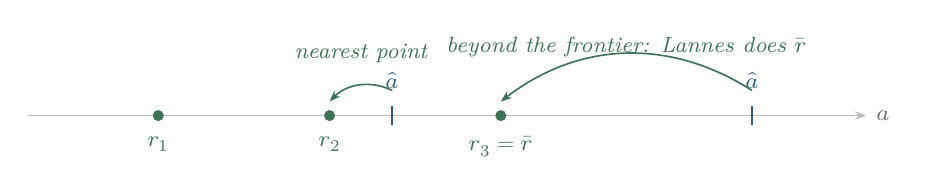
\begin{tikzpicture}
    \draw[hair,line width=0.5pt,-{Stealth[length=4pt]}] (-0.2,0) -- (10.440,0) node[right,font=\footnotesize,text=muted] {$a$};
    \fill[lan] (1.450,0) circle (2pt); \node[below=4pt,font=\footnotesize,text=lan] at (1.450,0) {$r_1$};
    \fill[lan] (3.625,0) circle (2pt); \node[below=4pt,font=\footnotesize,text=lan] at (3.625,0) {$r_2$};
    \fill[lan] (5.800,0) circle (2pt); \node[below=4pt,font=\footnotesize,text=lan] at (5.800,0) {$r_3=\bar r$};
    \draw[ber,line width=0.8pt] (4.422,-0.12) -- (4.422,0.12); \node[above=6pt,font=\footnotesize,text=ber] at (4.422,0) {$\hat a$};
    \draw[lan,line width=0.6pt,-{Stealth[length=4pt]}] (4.422,0.32) to[bend right=35] (3.625,0.18);
    \draw[ber,line width=0.8pt] (8.990,-0.12) -- (8.990,0.12); \node[above=6pt,font=\footnotesize,text=ber] at (8.990,0) {$\hat a$};
    \draw[lan,line width=0.6pt,-{Stealth[length=4pt]}] (8.990,0.32) to[bend right=35] (5.800,0.18);
    \node[font=\footnotesize\itshape,text=lan,anchor=south] at (7.395,0.62) {beyond the frontier: Lannes does $\bar r$};
    \node[font=\footnotesize\itshape,text=lan,anchor=south] at (4.024,0.55) {nearest point};
  \end{tikzpicture}\par
  \raggedright
  \vspace{0.8cm}
  \begin{keypoint}[lan]
    The \textbf{physical frontier} is $\bar r=\max\mathcal{R}$. Anything beyond it is done at $\bar r$.
  \end{keypoint}
\end{frame}

\begin{frame}{Better plans sit further out}
  A plan's ideal action measures its \tN{ambition}, and value rises with ambition:
  \[\textcolor{nap}{v(\xi)=\beta\,a^*(\xi)},\qquad\beta>0.\]
  The payoff is as before:
  \[W(a;\xi)=v(\xi)-\tfrac H2\big(a-a^*(\xi)\big)^2,\qquad H>0.\]
\end{frame}

\begin{frame}{Ambition beyond the frontier is wasted}
  \vspace{0.2cm}
  \centering
  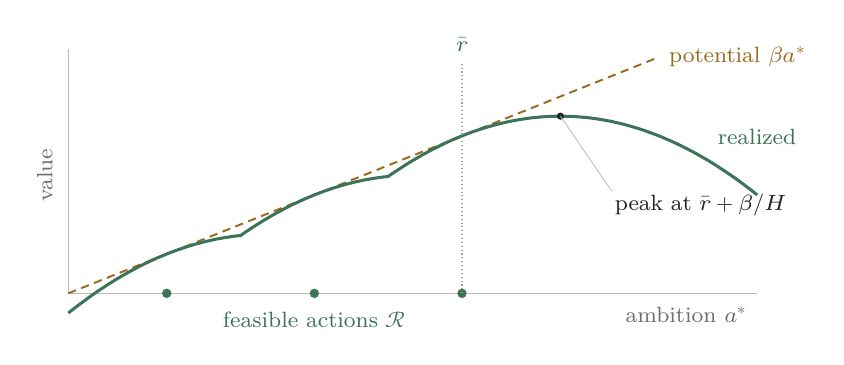
\begin{tikzpicture}
    \draw[hair,line width=0.4pt] (0,0) -- (8.750,0);
    \draw[hair,line width=0.4pt] (0,0) -- (0,3.100);
    \draw[densely dashed,nap,line width=0.7pt] (0,0) -- (7.500,3.000) node[anchor=west,font=\footnotesize,text=nap] {potential $\beta a^*$};
    \draw[lan,line width=1.1pt] plot coordinates {(0.000,-0.250) (0.062,-0.201) (0.125,-0.153) (0.188,-0.106) (0.250,-0.060) (0.312,-0.016) (0.375,0.028) (0.438,0.069) (0.500,0.110) (0.562,0.149) (0.625,0.188) (0.688,0.224) (0.750,0.260) (0.812,0.294) (0.875,0.328) (0.938,0.359) (1.000,0.390) (1.062,0.419) (1.125,0.448) (1.188,0.474) (1.250,0.500) (1.312,0.524) (1.375,0.547) (1.438,0.569) (1.500,0.590) (1.562,0.609) (1.625,0.628) (1.688,0.644) (1.750,0.660) (1.813,0.674) (1.875,0.688) (1.938,0.699) (2.000,0.710) (2.062,0.719) (2.125,0.728) (2.188,0.734) (2.250,0.778) (2.312,0.819) (2.375,0.860) (2.438,0.899) (2.500,0.938) (2.563,0.974) (2.625,1.010) (2.688,1.044) (2.750,1.078) (2.812,1.109) (2.875,1.140) (2.938,1.169) (3.000,1.198) (3.062,1.224) (3.125,1.250) (3.188,1.274) (3.250,1.298) (3.313,1.319) (3.375,1.340) (3.438,1.359) (3.500,1.378) (3.562,1.394) (3.625,1.410) (3.688,1.424) (3.750,1.438) (3.813,1.449) (3.875,1.460) (3.938,1.469) (4.000,1.478) (4.062,1.484) (4.125,1.528) (4.188,1.569) (4.250,1.610) (4.312,1.649) (4.375,1.688) (4.438,1.724) (4.500,1.760) (4.562,1.794) (4.625,1.828) (4.688,1.859) (4.750,1.890) (4.812,1.919) (4.875,1.948) (4.938,1.974) (5.000,2.000) (5.062,2.024) (5.125,2.048) (5.188,2.069) (5.250,2.090) (5.312,2.109) (5.375,2.127) (5.438,2.144) (5.500,2.160) (5.562,2.174) (5.625,2.188) (5.688,2.199) (5.750,2.210) (5.812,2.219) (5.875,2.228) (5.938,2.234) (6.000,2.240) (6.063,2.244) (6.125,2.248) (6.188,2.249) (6.250,2.250) (6.313,2.249) (6.375,2.248) (6.438,2.244) (6.500,2.240) (6.562,2.234) (6.625,2.228) (6.688,2.219) (6.750,2.210) (6.812,2.199) (6.875,2.188) (6.938,2.174) (7.000,2.160) (7.062,2.144) (7.125,2.127) (7.188,2.109) (7.250,2.090) (7.313,2.069) (7.375,2.047) (7.438,2.024) (7.500,2.000) (7.563,1.974) (7.625,1.947) (7.688,1.919) (7.750,1.890) (7.812,1.859) (7.875,1.827) (7.938,1.794) (8.000,1.760) (8.062,1.724) (8.125,1.688) (8.188,1.649) (8.250,1.610) (8.312,1.569) (8.375,1.527) (8.438,1.484) (8.500,1.440) (8.562,1.394) (8.625,1.347) (8.688,1.299) (8.750,1.250)};
    \node[anchor=south west,font=\footnotesize,text=lan] at (8.125,1.760) {realized};
    \fill[lan] (1.250,0) circle (1.7pt);
    \fill[lan] (3.125,0) circle (1.7pt);
    \fill[lan] (5.000,0) circle (1.7pt);
    \node[font=\footnotesize,text=lan,below=3pt] at (3.125,0) {feasible actions $\mathcal{R}$};
    \draw[lan!60,densely dotted] (5.000,0) -- (5.000,2.950) node[above,font=\footnotesize,text=lan] {$\bar r$};
    \fill[ink] (6.250,2.250) circle (1.3pt);
    \draw[hair,line width=0.3pt] (6.250,2.250) -- (6.900,1.300) node[anchor=north west,font=\footnotesize,text=ink,inner sep=1pt] {peak at $\bar r+\beta/H$};
    \node[font=\footnotesize,text=muted,anchor=north east] at (8.750,-0.05) {ambition $a^*$};
    \node[font=\footnotesize,text=muted,rotate=90] at (-0.3,1.500) {value};
  \end{tikzpicture}\par
  \raggedright
  \vspace{0.35cm}
  \aside{Napoleon's signals are about the realized curve, $U$, not the potential line, so he does not chase plans beyond the frontier.}
\end{frame}

\begin{frame}{Result 4: the physical frontier bounds output}
  \head{Proposition 4}
  {\itshape For any Napoleon, any Berthier, and any distribution of plans,}
  \[U,\ Y\ \le\ \beta\bar r+\frac{\beta^2}{2H}\qquad\text{and}\qquad\Ycal\ \le\ \mu_L\Big(\beta\bar r+\frac{\beta^2}{2H}\Big).\]
  \begin{keypoint}[lan]
    Even heavy-tailed plans cannot help: their tail lies beyond the frontier.
  \end{keypoint}
\end{frame}

\begin{frame}{Physical progress is a better \Lan}
  \head[lan]{Definition 7 (Physical progress)}
  \tL{Physical progress} is an improvement to Lannes:
  \[\mathcal{R}'\supseteq\mathcal{R}\qquad\text{or}\qquad\tau_L'\le\tau_L.\]
  \vspace{0.2cm}
  \begin{keypoint}[lan]
    It moves the frontier out, or raises capacity.
  \end{keypoint}
\end{frame}

\begin{frame}{Without physical progress, nothing grows}
  \head{Corollary}
  {\itshape If $\bar r$ and $\mu_L$ grow at most at rates $g_R$ and $g_L$, then for any AI and any vision}
  \[\limsup_{t\to\infty}\tfrac1t\ln\Ycal_t\ \le\ g_R+g_L.\]
  \begin{keypoint}[lan]
    No physical progress means no long-run growth, under AI, vision, or RSI.
  \end{keypoint}
\end{frame}

% ======================================================================= research
\begin{frame}{A research sector: \Nap{} and \Ber{} only}
  In \tK{research} nothing has to be built: \Nap{} picks the question and \Ber's solution \emph{is} the output.
  \[Y=W(\hat a;\xi),\qquad U=v(\xi)-\textcolor{ber}{\kappa_B(\xi)},\qquad K=\mu_B=\frac{n_B}{\tau_B}.\]
  \begin{keypoint}
    No budget set and no \Lan{} capacity: the only constraints are \textcolor{nap}{screening} and \textcolor{ber}{solving}.
  \end{keypoint}
  \vspace{0.2cm}
  \aside{Proofs, designs, software, simulations. Same model, with $\mathcal{R}=\mathcal{A}$ and $\mu_L=\infty$, so the best feasible value is $v(\xi)$ itself.}
\end{frame}

\begin{frame}{In research, AI relaxes \Nap's constraint}
  \Nap's capacity constraint is $Q(\pi)\le K$.
  \begin{itemize}\setlength{\itemsep}{6pt}
    \item \emph{Production}: $K=\min\{\mu_B,\mu_L\}\le\mu_L$. AI can lift $K$ only up to \Lan's capacity.
    \item \emph{Research}: $K=\mu_B$. AI lifts $K$ without limit.
  \end{itemize}
  \vspace{0.1cm}
  Since $Q(\pi)\le n_A/\tau_s$ for every policy, once $\mu_B\ge n_A/\tau_s$ the constraint never binds.
  \vspace{0.2cm}
  \begin{keypoint}[nap]
    \Nap{} stops rationing: he pursues every plan he expects to be worth something.
  \end{keypoint}
\end{frame}

\begin{frame}{Result 5: AI lifts research to \Nap's ceiling}
  \head{Proposition 5}
  {\itshape In research, fix \Nap. Along any path of AI, for all $t$,}
  \[\Ycal_t\ \le\ \frac{n_A}{\tau_s}\;\E_{\xi\sim F}\big[\max\{0,\ v(\xi)\}\big],\]
  {\itshape and once $\mu_{B,t}\ge n_A/\tau_s$, \Nap's capacity constraint is slack.}
  \begin{keypoint}[ber]
    AI makes \Nap{} the bottleneck. The ceiling depends only on how fast he can screen.
  \end{keypoint}
\end{frame}

\begin{frame}{Result 6: in research, RSI sustains growth}
  \head{Proposition 6}
  {\itshape In research with Gaussian plans, suppose AI raises capacity at rate $g_B$, $\mu_{B,t}=\mu_{B,0}e^{g_Bt}$, and vision speeds up screening at rate $g$, $\tau_{s,t}=\tau_{s,0}e^{-gt}$, without making signals noisier. Then}
  \[g_{\Ycal}=\min\{g_B,\ g\}.\]
  \begin{keypoint}
    Research grows when \emph{both} thinking constraints keep relaxing, even with thin tails.
  \end{keypoint}
  \vspace{0.15cm}
  \aside{AI alone ($g=0$) or vision alone ($g_B=0$) still gives zero growth: one constraint stays fixed.}
\end{frame}

\begin{frame}{Research versus production}
  \vspace{0.1cm}
  \centering
  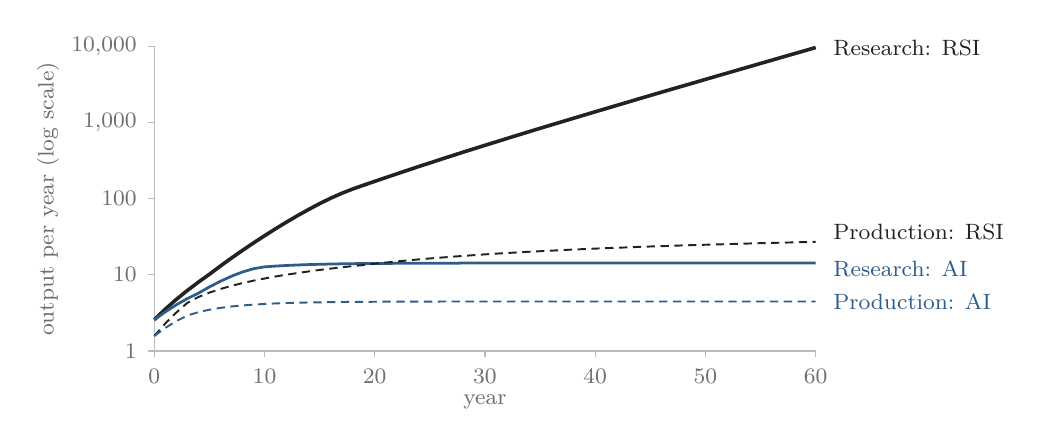
\begin{tikzpicture}
    \draw[hair,line width=0.4pt] (0,0) -- (0,3.868);
    \draw[hair,line width=0.4pt] (0,0) -- (8.400,0);
    \draw[hair,line width=0.4pt] (-0.08,0.000) -- (0,0.000); \node[anchor=east,font=\footnotesize,text=muted] at (-0.1,0.000) {1};
    \draw[hair,line width=0.4pt] (-0.08,0.967) -- (0,0.967); \node[anchor=east,font=\footnotesize,text=muted] at (-0.1,0.967) {10};
    \draw[hair,line width=0.4pt] (-0.08,1.934) -- (0,1.934); \node[anchor=east,font=\footnotesize,text=muted] at (-0.1,1.934) {100};
    \draw[hair,line width=0.4pt] (-0.08,2.901) -- (0,2.901); \node[anchor=east,font=\footnotesize,text=muted] at (-0.1,2.901) {1{,}000};
    \draw[hair,line width=0.4pt] (-0.08,3.868) -- (0,3.868); \node[anchor=east,font=\footnotesize,text=muted] at (-0.1,3.868) {10{,}000};
    \draw[hair,line width=0.4pt] (0.000,0) -- (0.000,-0.08); \node[anchor=north,font=\footnotesize,text=muted] at (0.000,-0.1) {0};
    \draw[hair,line width=0.4pt] (1.400,0) -- (1.400,-0.08); \node[anchor=north,font=\footnotesize,text=muted] at (1.400,-0.1) {10};
    \draw[hair,line width=0.4pt] (2.800,0) -- (2.800,-0.08); \node[anchor=north,font=\footnotesize,text=muted] at (2.800,-0.1) {20};
    \draw[hair,line width=0.4pt] (4.200,0) -- (4.200,-0.08); \node[anchor=north,font=\footnotesize,text=muted] at (4.200,-0.1) {30};
    \draw[hair,line width=0.4pt] (5.600,0) -- (5.600,-0.08); \node[anchor=north,font=\footnotesize,text=muted] at (5.600,-0.1) {40};
    \draw[hair,line width=0.4pt] (7.000,0) -- (7.000,-0.08); \node[anchor=north,font=\footnotesize,text=muted] at (7.000,-0.1) {50};
    \draw[hair,line width=0.4pt] (8.400,0) -- (8.400,-0.08); \node[anchor=north,font=\footnotesize,text=muted] at (8.400,-0.1) {60};
    \draw[ink,line width=1.3pt] plot coordinates {(0.000,0.396) (0.140,0.531) (0.280,0.655) (0.420,0.768) (0.560,0.874) (0.700,0.974) (0.840,1.079) (0.980,1.180) (1.120,1.277) (1.260,1.372) (1.400,1.463) (1.540,1.552) (1.680,1.637) (1.820,1.719) (1.960,1.797) (2.100,1.871) (2.240,1.940) (2.380,2.002) (2.520,2.057) (2.660,2.106) (2.800,2.154) (2.940,2.202) (3.080,2.249) (3.220,2.296) (3.360,2.343) (3.500,2.388) (3.640,2.434) (3.780,2.479) (3.920,2.524) (4.060,2.568) (4.200,2.612) (4.340,2.655) (4.480,2.699) (4.620,2.742) (4.760,2.785) (4.900,2.828) (5.040,2.870) (5.180,2.912) (5.320,2.954) (5.460,2.996) (5.600,3.038) (5.740,3.079) (5.880,3.121) (6.020,3.162) (6.160,3.204) (6.300,3.245) (6.440,3.286) (6.580,3.327) (6.720,3.367) (6.860,3.408) (7.000,3.449) (7.140,3.490) (7.280,3.530) (7.420,3.571) (7.560,3.611) (7.700,3.652) (7.840,3.692) (7.980,3.733) (8.120,3.773) (8.260,3.813) (8.400,3.854)};
    \node[anchor=west,font=\footnotesize,text=ink] at (8.500,3.854) {Research: RSI};
    \draw[ber,line width=1.0pt] plot coordinates {(0.000,0.396) (0.140,0.496) (0.280,0.586) (0.420,0.665) (0.560,0.734) (0.700,0.813) (0.840,0.885) (0.980,0.949) (1.120,1.003) (1.260,1.045) (1.400,1.068) (1.540,1.078) (1.680,1.086) (1.820,1.092) (1.960,1.097) (2.100,1.101) (2.240,1.104) (2.380,1.107) (2.520,1.109) (2.660,1.110) (2.800,1.111) (2.940,1.112) (3.080,1.113) (3.220,1.114) (3.360,1.114) (3.500,1.115) (3.640,1.115) (3.780,1.115) (3.920,1.116) (4.060,1.116) (4.200,1.116) (4.340,1.116) (4.480,1.116) (4.620,1.116) (4.760,1.116) (4.900,1.116) (5.040,1.116) (5.180,1.116) (5.320,1.116) (5.460,1.116) (5.600,1.116) (5.740,1.116) (5.880,1.116) (6.020,1.116) (6.160,1.116) (6.300,1.116) (6.440,1.116) (6.580,1.117) (6.720,1.117) (6.860,1.117) (7.000,1.117) (7.140,1.117) (7.280,1.117) (7.420,1.117) (7.560,1.117) (7.700,1.117) (7.840,1.117) (7.980,1.117) (8.120,1.117) (8.260,1.117) (8.400,1.117)};
    \node[anchor=west,font=\footnotesize,text=ber] at (8.500,1.037) {Research: AI};
    \draw[densely dashed,ink,line width=0.7pt] plot coordinates {(0.000,0.190) (0.140,0.349) (0.280,0.488) (0.420,0.611) (0.560,0.685) (0.700,0.741) (0.840,0.787) (0.980,0.827) (1.120,0.862) (1.260,0.893) (1.400,0.920) (1.540,0.946) (1.680,0.969) (1.820,0.990) (1.960,1.010) (2.100,1.029) (2.240,1.046) (2.380,1.063) (2.520,1.078) (2.660,1.092) (2.800,1.108) (2.940,1.123) (3.080,1.137) (3.220,1.150) (3.360,1.163) (3.500,1.175) (3.640,1.186) (3.780,1.197) (3.920,1.207) (4.060,1.217) (4.200,1.227) (4.340,1.236) (4.480,1.244) (4.620,1.252) (4.760,1.260) (4.900,1.267) (5.040,1.274) (5.180,1.281) (5.320,1.288) (5.460,1.294) (5.600,1.300) (5.740,1.306) (5.880,1.311) (6.020,1.316) (6.160,1.322) (6.300,1.327) (6.440,1.331) (6.580,1.336) (6.720,1.341) (6.860,1.345) (7.000,1.349) (7.140,1.353) (7.280,1.357) (7.420,1.361) (7.560,1.365) (7.700,1.369) (7.840,1.372) (7.980,1.376) (8.120,1.379) (8.260,1.383) (8.400,1.386)};
    \node[anchor=west,font=\footnotesize,text=ink] at (8.500,1.506) {Production: RSI};
    \draw[densely dashed,ber,line width=0.7pt] plot coordinates {(0.000,0.190) (0.140,0.292) (0.280,0.380) (0.420,0.450) (0.560,0.493) (0.700,0.524) (0.840,0.547) (0.980,0.565) (1.120,0.578) (1.260,0.589) (1.400,0.597) (1.540,0.604) (1.680,0.609) (1.820,0.613) (1.960,0.616) (2.100,0.618) (2.240,0.620) (2.380,0.622) (2.520,0.623) (2.660,0.624) (2.800,0.625) (2.940,0.626) (3.080,0.626) (3.220,0.627) (3.360,0.627) (3.500,0.627) (3.640,0.628) (3.780,0.628) (3.920,0.628) (4.060,0.628) (4.200,0.628) (4.340,0.628) (4.480,0.628) (4.620,0.628) (4.760,0.628) (4.900,0.628) (5.040,0.628) (5.180,0.628) (5.320,0.628) (5.460,0.628) (5.600,0.628) (5.740,0.628) (5.880,0.628) (6.020,0.628) (6.160,0.628) (6.300,0.628) (6.440,0.628) (6.580,0.628) (6.720,0.628) (6.860,0.628) (7.000,0.628) (7.140,0.628) (7.280,0.628) (7.420,0.628) (7.560,0.628) (7.700,0.628) (7.840,0.628) (7.980,0.628) (8.120,0.628) (8.260,0.628) (8.400,0.628)};
    \node[anchor=west,font=\footnotesize,text=ber] at (8.500,0.628) {Production: AI};
    \node[font=\footnotesize,text=muted] at (4.2,-0.65) {year};
    \node[font=\footnotesize,text=muted,rotate=90] at (-1.35,1.93) {output per year (log scale)};
  \end{tikzpicture}\par
  \raggedright
  \vspace{0.2cm}
  \aside{Same parameters as the illustration; research drops Lannes ($\kappa_L=0$, no capacity cap).}
\end{frame}

\begin{frame}{What changes in research}
  \centering
  \renewcommand{\arraystretch}{1.2}
  \begin{tabular}{@{}l r r r r@{}}
    \toprule
    & \multicolumn{2}{c}{Production} & \multicolumn{2}{c}{Research} \\
    \cmidrule(lr){2-3}\cmidrule(lr){4-5}
    & Year 60 & Growth & Year 60 & Growth \\
    \midrule
    \textcolor{ber}{AI} & 4.47 & 0\% & 14.27 & 0\% \\
    \textcolor{nap}{Vision} & 12.75 & 0.9\% & 13.75 & 0.8\% \\
    RSI & 27.12 & 0.9\% & 9{,}654 & 10.1\% \\
    \bottomrule
  \end{tabular}\par
  \raggedright
  \vspace{0.3cm}
  \begin{itemize}\setlength{\itemsep}{3pt}
    \item With AI, \Nap{} goes from accepting 1 plan a year to 10, and from 3 signals per plan to 1.
    \item With RSI, research output grows at the screening rate, about $10\%$ a year.
  \end{itemize}
  \vspace{0.1cm}
  \aside{Growth over years 50--60. Year 0 output is 1.57 in production and 2.57 in research.}
\end{frame}

% ======================================================================= summary
\begin{frame}{Summary}
  \begin{keypoint}[ber]
    AI raises the level of output, not its growth rate.
  \end{keypoint}
  \vspace{0.2cm}
  \begin{keypoint}[nap]
    Sharper judgment has a ceiling; faster screening sustains growth only if plan values are heavy-tailed.
  \end{keypoint}
  \vspace{0.2cm}
  \begin{keypoint}[lan]
    The physical frontier bounds output, whatever thinking does.
  \end{keypoint}
  \vspace{0.2cm}
  \vspace{0.2cm}
  \begin{keypoint}
    In research, AI relaxes Napoleon's constraint, and RSI can sustain growth.
  \end{keypoint}
  \vspace{0.2cm}
  \begin{keypoint}
    In production, lasting growth needs physical progress.
  \end{keypoint}
\end{frame}

% ======================================================================= appendix
{\setbeamertemplate{footline}{}
\begin{frame}[plain,c]
  \hspace*{0.2cm}{\fontsize{24}{28}\selectfont Appendix}
\end{frame}}

\begin{frame}{Computing $Q$: the acceptance probability}
  Write $s_{1:n}=(s_1,\dots,s_n)$ and $P_u^n(ds_{1:n})=\prod_{k=1}^nP(ds_k\mid u)$. Napoleon accepts at signal $n$ on
  \[A_n=\big\{s_{1:n}:\ \pi_j(s_{1:j})=\text{wait for all }j<n,\ \ \pi_n(s_{1:n})=\text{accept}\big\}.\]
  These events are disjoint, so
  \[P_\pi(\text{accept}\mid u)=\sum_{n\ge1}P_u^n(A_n),\qquad P_\pi(\text{accept})=\int P_\pi(\text{accept}\mid u)\,dG(u).\]
  \aside{$P_\pi(\text{accept}\mid u)$ is the chance a plan of value $u$ is accepted; sharper signals make it rise more steeply in $u$.}
\end{frame}

\begin{frame}{Computing $Q$: the length of an investigation}
  Napoleon is still waiting after $m$ signals on
  \[W_m=\big\{s_{1:m}:\ \pi_j(s_{1:j})=\text{wait for all }j\le m\big\},\qquad W_0=\text{everything}.\]
  He takes an $n$-th signal exactly when he waited through the first $n-1$, so
  \[\E_\pi[N_\pi]=\sum_{n\ge1}P_\pi(N_\pi\ge n)=\sum_{n\ge1}\int P_u^{\,n-1}(W_{n-1})\,dG(u).\]
  \aside{One investigation takes $\tau_s N_\pi$ units of time, $\tau_s\E_\pi[N_\pi]$ on average.}
\end{frame}

\begin{frame}{Computing $Q$: putting it together}
  Each Napoleon examines independent plans one after another. By the renewal--reward theorem,
  \[\lim_{T\to\infty}\frac{\#\{\text{plans examined by }T\}}{T}=\frac{1}{\tau_s\,\E_\pi[N_\pi]}.\]
  A share $P_\pi(\text{accept})$ is accepted, and $n_A$ Napoleons work in parallel:
  \[Q(\pi)=\underset{\text{Napoleons}}{n_A}\ \times\underset{\text{plans examined each}}{\frac{1}{\tau_s\,\E_\pi[N_\pi]}}\times\ \underset{\text{share accepted}}{P_\pi(\text{accept})}.\]
  \begin{keypoint}[nap]
    Waiting longer raises $\E_\pi[N_\pi]$: better information, but fewer plans examined.
  \end{keypoint}
\end{frame}

\begin{frame}{Computing $Q$: the value of accepted plans}
  The same objects give the objective in Problem N:
  \[\E_\pi[U\mid\text{accept}]=\frac{\int u\,P_\pi(\text{accept}\mid u)\,dG(u)}{P_\pi(\text{accept})},\]
  so output is
  \[\Ycal(\pi)=Q(\pi)\,\E_\pi[U\mid\text{accept}]=\frac{n_A}{\tau_s\,\E_\pi[N_\pi]}\int u\,P_\pi(\text{accept}\mid u)\,dG(u).\]
\end{frame}

\begin{frame}{The renewal--reward theorem}
  Suppose a process splits into independent cycles: cycle $i$ lasts $T_i$ and earns $R_i$, with $(T_i,R_i)$ i.i.d.\ and $\E[T]<\infty$. Then almost surely
  \[\lim_{t\to\infty}\frac{\text{reward earned by }t}{t}=\frac{\E[R]}{\E[T]}.\]
  \emph{Why.} By the law of large numbers, about $t/\E[T]$ cycles finish by time $t$, and their average reward tends to $\E[R]$.
  \vspace{0.2cm}

  \head{Applied to Napoleon}
  One cycle is one investigation, $T_i=\tau_sN_i$. Reward $1$ counts plans examined; reward $\mathbf{1}\{\text{accept}\}$ counts plans accepted; reward $U_i\mathbf{1}\{\text{accept}\}$ gives output.
\end{frame}

\begin{frame}{Proof of Lemma 1}
  Write $\varepsilon=\varepsilon_B$. Because $|\hat W-W|\le\varepsilon$ everywhere and $\hat a$ maximizes $\hat W$,
  \[W(\hat a;\xi)\ \ge\ \hat W(\hat a;\xi)-\varepsilon\ \ge\ \hat W\big(a^*(\xi);\xi\big)-\varepsilon\ \ge\ W\big(a^*(\xi);\xi\big)-2\varepsilon.\]
  So $\kappa_B=|v(\xi)-W(\hat a;\xi)|\le2\varepsilon$. The rate $\varepsilon\le C_sk^{-s/d}$ is a Jackson-type bound for polynomial and spline sieves. \hfill$\square$
\end{frame}

\begin{frame}{Lemma 3}
  \head{Statement}
  {\itshape For any policy, output is bounded by the rate of screening: $\Ycal\le\bar R\,\E[U^+]$, where $\bar R=n_A/\tau_s$.}
  \vspace{0.4cm}

  \emph{Proof.} Each plan needs at least one signal, so plans are examined at rate $R\le\bar R$. With $A=\{\text{accept}\}$,
  \[\Ycal=Q\,\E[U\mid A]=R\,\E[U\mathbf{1}_A]\ \le\ \bar R\,\E[U^+].\qquad\square\]
\end{frame}

\begin{frame}{Proof of Proposition 1}
  \begin{itemize}\setlength{\itemsep}{8pt}
    \item Whatever Berthier does, the realized action lies in $\mathcal{R}$, so $Y\le\bar U(\xi)$ and hence $U_t\le\bar U$.
    \item By Lemma 3, $\Ycal_t\le\bar R\,\E[U_t^+]\le\bar R\,\E[\bar U^+]$.
    \item $\bar U\le v$, so $\E[\bar U^+]\le\E[v^+]<\infty$.
    \item A bounded sequence has $\limsup_t\tfrac1t\ln\Ycal_t\le0$. \hfill$\square$
  \end{itemize}
\end{frame}

\begin{frame}{Proof of Lemma 2}
  Let $X=Z-\E[Z]$. For any $\theta>0$, Jensen's inequality gives
  \[e^{\theta\E[X\mid A]}\ \le\ \E\big[e^{\theta X}\mid A\big]\ \le\ \frac{\E\big[e^{\theta X}\big]}{q}.\]
  Take logs and use $\ln\E[e^{\theta X}]\le\theta^2\sigma^2/2$:
  \[\E[X\mid A]\ \le\ \frac{\theta\sigma^2}{2}+\frac{\ln(1/q)}{\theta}.\]
  Choose $\theta=\sqrt{2\ln(1/q)}/\sigma$. \hfill$\square$
\end{frame}

\begin{frame}{Proof of Proposition 2}
  Accepted plans flow at $Q=qR\le K$, with $R\le\bar R$. Since $U\le\bar U$, Lemma 2 with $Z=\bar U$ gives
  \[\Ycal=Q\,\E[U\mid A]\ \le\ Q\,\E[\bar U\mid A]\ \le\ Q\,\bar m^++\sigma f(Q,R),\qquad f(Q,R)=Q\sqrt{2\ln(R/Q)}.\]
  \begin{itemize}\setlength{\itemsep}{6pt}
    \item $f$ is increasing in $R$, and in $Q$ when $Q\le R/\sqrt e$.
    \item With $R\le\bar R$ and $Q\le K\le\bar R/\sqrt e$: $f\le K\sqrt{2\ln(\bar R/K)}$. \hfill$\square$
  \end{itemize}
\end{frame}

\begin{frame}{Proof of Proposition 3}
  \begin{itemize}\setlength{\itemsep}{8pt}
    \item Proposition 2 holds at each date $t$, for any Berthier.
    \item Its bound rises with $K$ (for $K\le\bar R_t/\sqrt e$), so use $K_t\le\mu_L$.
    \item Substitute $\bar R_t\le\bar R_0e^{gt}$.
    \item A bound of order $\sqrt t$ implies $\limsup_t\tfrac1t\ln\Ycal_t\le0$. \hfill$\square$
  \end{itemize}
\end{frame}

\begin{frame}{Proof of the heavy-tail result}
  \begin{itemize}\setlength{\itemsep}{8pt}
    \item No policy beats perfect sorting: $\E[U\mid\text{accept}]\le M(q)$, the mean of the top share $q$ of $U$.
    \item For a Pareto tail, $M(q)=\tfrac{\alpha}{\alpha-1}x_mq^{-1/\alpha}$.
    \item So $\Ycal_t\le\mu_L\,M(\mu_L/\bar R_t)$, which grows at rate at most $g/\alpha$.
    \item With perfectly informative signals Napoleon sorts perfectly, so $\Ycal_t=K\,M(K/\bar R_t)$, which grows at exactly $g/\alpha$. \hfill$\square$
  \end{itemize}
\end{frame}

\begin{frame}{Proof of Proposition 4}
  \begin{itemize}\setlength{\itemsep}{8pt}
    \item The realized action is some $r\in\mathcal{R}$, so $r\le\bar r$; the bound on $Y$ then also holds for its expectation $U$.
    \item For fixed $r$, $\beta a^*-\tfrac H2(r-a^*)^2$ is largest at $a^*=r+\beta/H$, so
    \[Y\ \le\ \beta r+\frac{\beta^2}{2H}\ \le\ \beta\bar r+\frac{\beta^2}{2H}.\]
    \item At most $\mu_L$ plans are carried out per unit of time. \hfill$\square$
  \end{itemize}
\end{frame}

\begin{frame}{Proof of Proposition 5}
  \begin{itemize}\setlength{\itemsep}{8pt}
    \item In research $U=v-\kappa_B\le v$, because $\kappa_B\ge0$.
    \item By Lemma 3, $\Ycal_t\le\frac{n_A}{\tau_s}\E[U_t^+]\le\frac{n_A}{\tau_s}\E[v^+]$, whatever Berthier does.
    \item Each plan needs at least one signal, so every policy has $Q(\pi)\le R(\pi)\le n_A/\tau_s$. If $\mu_{B,t}\ge n_A/\tau_s$, then $Q(\pi)\le K_t$ for every policy: the constraint is slack. \hfill$\square$
  \end{itemize}
\end{frame}

\begin{frame}{Proof of Proposition 6}
  Write $\bar R_t=n_A/\tau_{s,t}$ and $K_t=\mu_{B,t}$; research means $\bar U=v\sim N(m,\sigma^2)$.
  \begin{itemize}\setlength{\itemsep}{4pt}
    \item \emph{Upper bound.} Lemma 3 gives $\Ycal_t\le\bar R_t\E[v^+]$, growing at rate $g$. If $g_B<g$, then $\bar R_t\ge\sqrt e K_t$ eventually and Proposition 2 gives $\Ycal_t\le K_t\big(m^++\sigma\sqrt{2\ln(\bar R_t/K_t)}\big)$, growing at rate $g_B$. So $g_{\Ycal}\le\min\{g_B,g\}$.
    \item \emph{Lower bound.} Take one signal and accept iff $\mu_1\ge\max\{c,z_t\}$, for a fixed $c>0$ and the capacity cutoff $z_t$. Accepted plans have $\E[U\mid\text{accept}]\ge c$, and $P(\mu_1\ge c)\ge p>0$ for all $t$, since AI only raises $m_U$ and signals do not get noisier. So $\Ycal_t\ge c\,\min\{\bar R_tp,\ K_t\}$, growing at rate $\min\{g,g_B\}$. \hfill$\square$
  \end{itemize}
\end{frame}

\end{document}
